\documentclass{ctexbeamer}
% This part is required to have NJU custom style
\usetheme[presentation]{nju}
\usecolortheme[presentation]{njucolor}
% Uncomment the next line if you want your itemize items to appear as a bullet, instead of triangular shapes
\usefonttheme[onlymath]{serif}
\renewcommand{\familydefault}{\rmdefault}
\usepackage[style=verbose, backend=bibtex]{biblatex}
\addbibresource{ref.bib}
%\setbeamertemplate{itemize item}{$\bullet$}

% Include the required packages here
\usepackage{graphicx,booktabs,tikz,pgfplots,amsfonts,amsmath,amsthm,hyperref,caption,newtxmath,amssymb}

% Tikz Customization
\usetikzlibrary{intersections}
\usepgfplotslibrary{fillbetween}

% PGFPlots config
\pgfplotsset{compat=1.14}

% cite command
\let\oldcite\cite
\renewcommand{\cite}[1]{\footcite{#1}}


% Logo in the first page, comment out if don't wanted
\presentationlogo{
\includegraphics[width=2cm]{logo/NJU-logo.jpg}}
%%%%%%%%%%%%%%%%%%%%%%%%%%%%%%%%%%%%%%%%%%%%%%%%%%%%%%%
\title[AI Foundations]{Mathematical Foundations of Artificial Intelligence}
\author[Li]{Eric Li}
\institute{School of Artificial Intelligence, Nanjing University}
\date{\today}
%%%%%%%%%%%%%%%%%%%%%%%%%%%%%%%%%%%%%%%%%%%%%%%%%%%%%%%
\begin{document}

% title page
\maketitle

% Intro section
\section{Introduction}
% A subsection. May contain multiple subsections
\subsection{Artificial Intelligence}
\begin{frame}{What is Artificial Intelligence?}
    This template is modified from the original FSU template by Rafiq Islam\cite{fsumathposter25} to create an NJU AI School presentation template\cite{njubeamerpresent25}. Here is how you use plain text. Here is how you can use a block to write some important information.
    \begin{block}{Artificial Intelligence}
        Artificial Intelligence is the study and design of intelligent agents that can perceive their environment and take actions to maximize their chances of success. Modern AI encompasses machine learning, deep learning, natural language processing, computer vision, and robotics.
    \end{block}
\end{frame}
\begin{frame}
    \frametitle{Example of itemize and enumerate}
    \begin{columns}[c, onlytextwidth]
        \begin{column}{0.48\textwidth}
            \small
            \begin{block}{AI Research Areas}
                \begin{itemize}
                    \item Machine Learning and Deep Learning
                    \item Natural Language Processing (NLP)
                    \item Computer Vision and Pattern Recognition
                    \item Robotics and Autonomous Systems
                    \item 人工智能算法与理论 (Chinese example)
                \end{itemize}
            \end{block}
        \end{column}
        \begin{column}{0.48\textwidth}
            \begin{block}{Key Technologies}
                \begin{enumerate}
                    \item Neural Networks and Deep Learning
                    \item Reinforcement Learning
                    \item Knowledge Representation and Reasoning
                    \item Computer Vision Systems
                \end{enumerate}
            \end{block}
        \end{column}
    \end{columns}
\end{frame}
%%%%%%%%%%%%%%%%%%%%%%%%%%%%%%%%%%%%%%%%%%%%%%%%%%
\subsection{Why Artificial Intelligence}
\begin{frame}{Why Artificial Intelligence?}
This template is modified from the original FSU template\footnote{Based on FSU Mathematics template by Rafiq Islam}. Artificial Intelligence is transforming industries and society by enabling machines to perform tasks that typically require human intelligence, such as visual perception, speech recognition, decision-making, and language translation.
\end{frame}
%%%%%%%%%%%%%%%%%%%%%%%%%%%%%%%%%%%
\section{Methodology}
\begin{frame}{Mathematical Foundations}
    This section covers the mathematical background of AI.\\
    The fundamental equation for neural networks is the forward propagation:
        \[
        a^{(l)} = \sigma(W^{(l)}a^{(l-1)} + b^{(l)})
        \]
    where $\sigma$ is the activation function, $W^{(l)}$ are the weights, and $b^{(l)}$ are the biases at layer $l$.
    \begin{enumerate}
        \item Backpropagation uses gradient descent to optimize network parameters.
        \item Convolutional Neural Networks (CNNs) excel in image processing tasks.
        \item Recurrent Neural Networks (RNNs) handle sequential data effectively.
    \end{enumerate}
\end{frame}
%%%%%%%%%%%%%%%%%%%%%%%%%%%%%%%%%%%%%%%%%%%
\begin{frame}{Neural Network Architecture}
    \begin{figure}
        \centering
        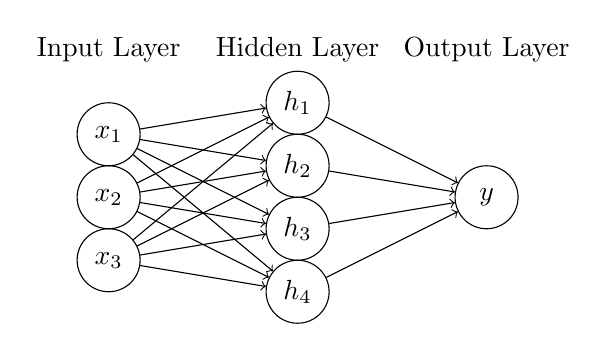
\begin{tikzpicture}[scale=0.8]
            % Input layer
            \foreach \i in {1,...,3}
                \node[circle,draw,minimum size=0.8cm] (input\i) at (0,-\i) {$x_\i$};
            
            % Hidden layer
            \foreach \i in {1,...,4}
                \node[circle,draw,minimum size=0.8cm] (hidden\i) at (3,-\i+0.5) {$h_\i$};
            
            % Output layer
            \node[circle,draw,minimum size=0.8cm] (output) at (6,-2) {$y$};
            
            % Connections
            \foreach \i in {1,...,3}
                \foreach \j in {1,...,4}
                    \draw[->] (input\i) -- (hidden\j);
            
            \foreach \i in {1,...,4}
                \draw[->] (hidden\i) -- (output);
            
            % Labels
            \node[above] at (0,0) {Input Layer};
            \node[above] at (3,0) {Hidden Layer};
            \node[above] at (6,0) {Output Layer};
        \end{tikzpicture}
        \caption{Basic Neural Network Architecture with 3 input neurons, 4 hidden neurons, and 1 output neuron}
        \label{fig:nn_arch}
    \end{figure}
\end{frame}
%%%%%%%%%%%%%%%%%%%%%%%
\begin{frame}{AI Applications}
    \begin{figure}
    \centering
    
\includegraphics[width=0.5\linewidth]{images/lamda.png}
    \caption{Nanjing University LAMDA Research Team (Photo credit: \href{https://lamda.nju.edu.cn/}{LAMDA})}
    \label{fig:ai_apps}
    \end{figure}
    \begin{itemize}
        \item Healthcare: Medical image analysis and diagnosis
        \item Transportation: Autonomous vehicles and traffic optimization
        \item Education: Personalized learning systems
        \item Finance: Fraud detection and algorithmic trading
    \end{itemize}
\end{frame}
%%%%%%%%%%%%%%%%%%%%%%%%%%%%%%%%%%%%%%
\section{Reference}
\begin{frame}[allowframebreaks]{Bibliography}
    \printbibliography
\end{frame}
\end{document}
